% it/figures/data_pipeline/fig_ews.tex — versione italiana
\begin{figure}[!ht]
    \centering
    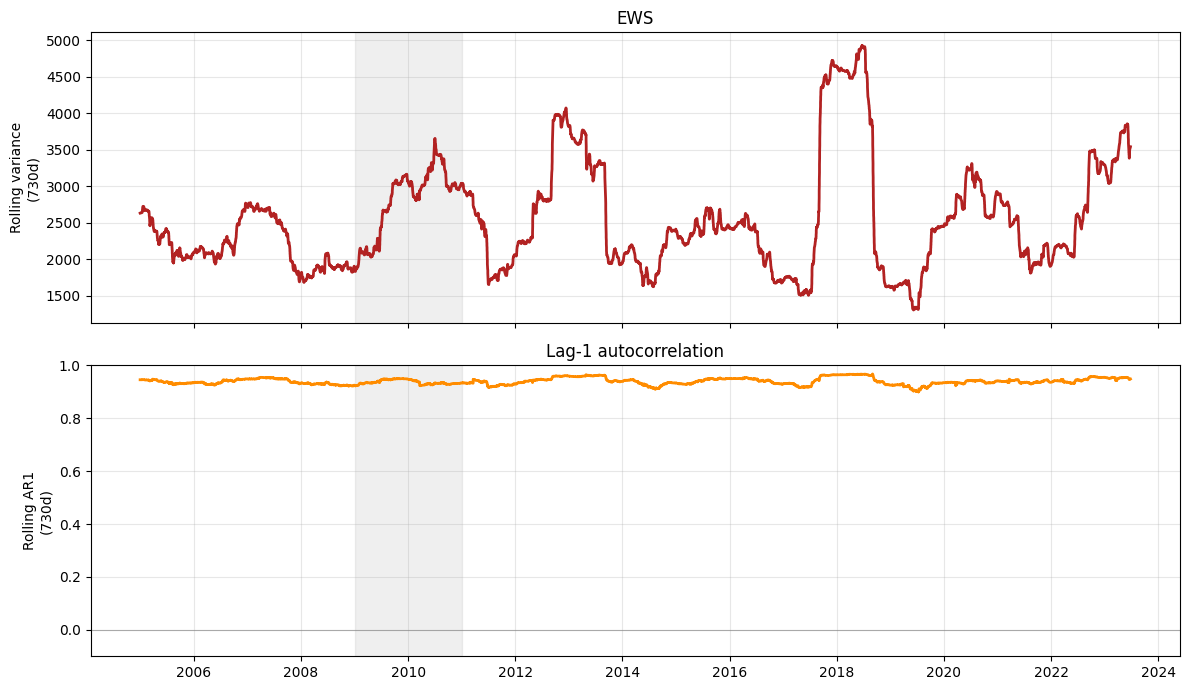
\includegraphics[width=0.9\textwidth]{figures/data_pipeline/ews.png}
    \caption[Segnali di preallarme: varianza mobile e autocorrelazione.]{\textbf{Nessun
    trend di preallarme rigoroso.} Varianza mobile e autocorrelazione a lag~1 della serie
    di intensità lungo il record. Entrambe oscillano senza una salita sostenuta.
    I loro p-value di trend ingenui ($\sim$$10^{-42}$) sono artefatti di finestre
    fortemente sovrapposte; corretti per le $\sim$19.5 finestre indipendenti che il
    record contiene davvero, i trend non sono significativi (p~$=$~0.634 e
    0.595; Tabella~\ref{tab:ews}).}
    \label{fig:ews}
\end{figure}
